\documentclass[aspectratio=169]{beamer}

\usepackage[utf8]{inputenc}
\usepackage{array}
\usepackage{booktabs}
\usepackage{graphics}
\usepackage{hyperref}
\hypersetup{%
  colorlinks=true,
  linkcolor=blue,
  filecolor=blue,
  urlcolor=cyan,
}
\usepackage{setspace}
\usepackage{verbatim}
\usepackage{fancyvrb} % for verbatim centering

\usetheme{Warsaw}
\usecolortheme{beaver}
\definecolor{clOrange}{HTML}{E76600}
\definecolor{clAlmostWhite}{HTML}{FEFFD9}
\definecolor{clGreen}{HTML}{2aa198}
\definecolor{clFlag}{HTML}{D33682}
\definecolor{clFlagOpt}{HTML}{CB4B16}
\definecolor{clRedFlag}{HTML}{DC322F}

\title[LTN02 :: CompilationFlags]{A quick look at C++ compilation flags}
\author{Adam Graliński}
\date[FFFE\_21]{\textbf{C++ {\color{red}F}{\color{blue}F}{\color{green}F}{\color{yellow}E}, February 2021}}

\setbeamertemplate{navigation symbols}{}
\setbeamercolor{title}{fg=black}
\setbeamercolor{author}{fg=clAlmostWhite}
\setbeamercolor{date}{fg=clAlmostWhite}
\setbeamerfont{author}{size=\huge}
\setbeamerfont{date}{size=\Large}

\begin{document}

{\usebackgroundtemplate{%
 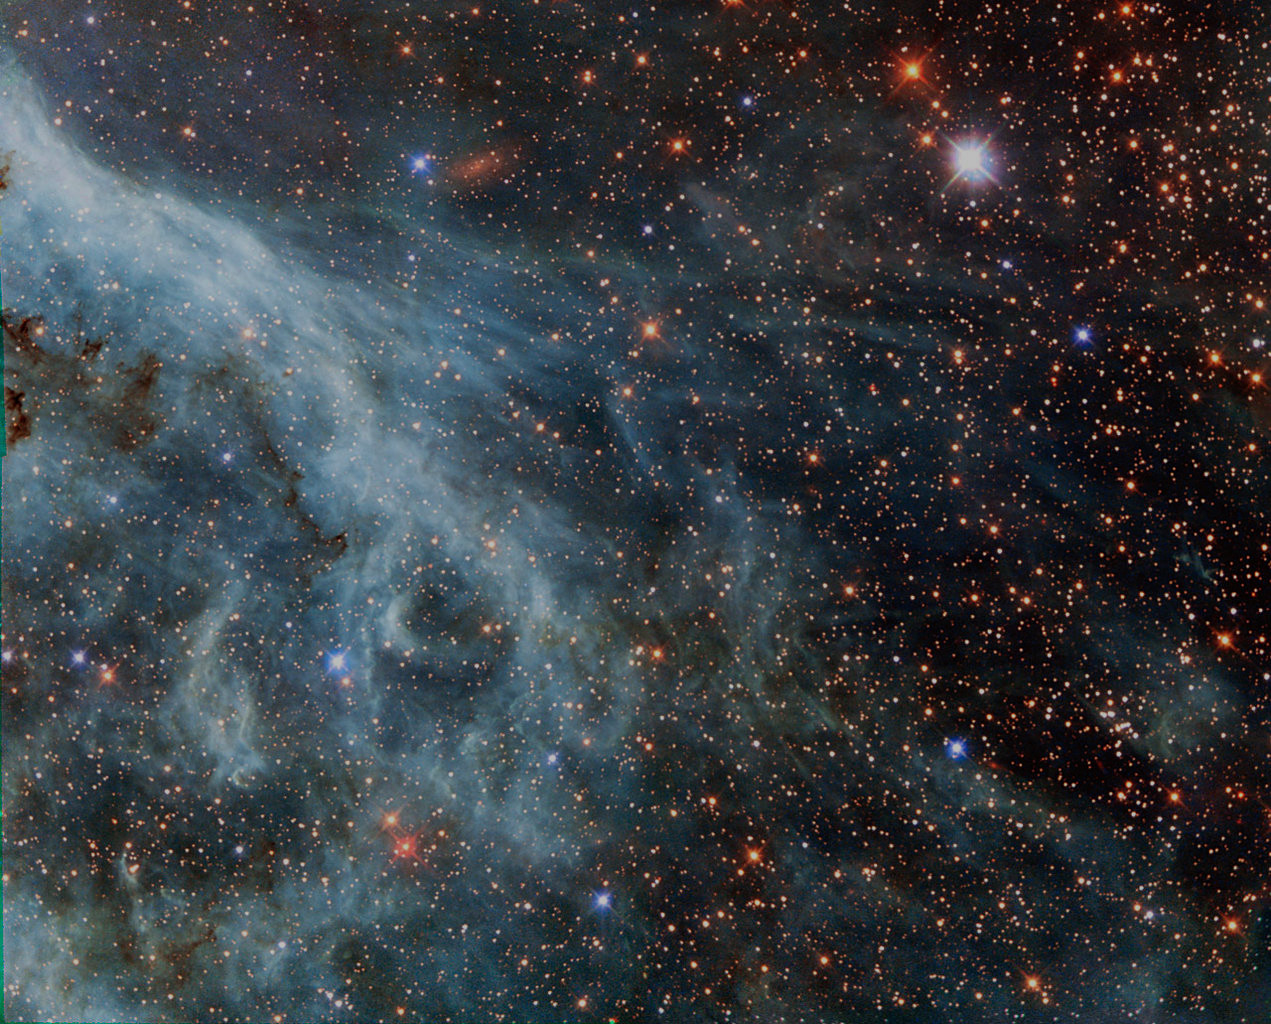
\includegraphics[width=\paperwidth,height=\paperheight]{../common/bg_galaxy.jpg}}
\begin{frame}
\titlepage{}
\end{frame}
}

\begin{frame}[fragile]
\frametitle{Flags}
\centering
\begin{center}{\huge {\color{clGreen}The Easy Part}}\end{center}
\vspace{1ex}
\begin{BVerbatim}[commandchars=\\\{\}]
g++ [\textcolor{clFlag}{-c}|\textcolor{clFlag}{-S}|\textcolor{clFlag}{-E}] [\textcolor{clFlag}{-std=}\textcolor{clFlagOpt}{standard}]
    [\textcolor{clFlag}{-g}] [\textcolor{clFlag}{-pg}] [\textcolor{clFlag}{-O}\textcolor{clFlagOpt}{level}]
    [-Wwarn...] [-Wpedantic]
    [\textcolor{clFlag}{-I}\textcolor{clFlagOpt}{dir...}] [\textcolor{clFlag}{-L}\textcolor{clFlagOpt}{dir...}]
    [\textcolor{clFlag}{-D}\textcolor{clFlagOpt}{macro[=defn]...}] [\textcolor{clFlag}{-U}\textcolor{clFlagOpt}{macro}]
    [-foption...] [-mmachine-option...]
    [\textcolor{clFlag}{-o} outfile] [\textcolor{clFlag}{@}\textcolor{clFlag}{file}] infile...
\end{BVerbatim}
\end{frame}

\begin{frame}
\frametitle{-c, -S, -E : stop after build phase}
\begin{table}
\begin{tabular}{l l}
\toprule
\texttt{\color{clFlag}{-E}} & stop after preprocessing step --- do not compile \\ [3ex]
\texttt{\color{clFlag}{-S}} & stop after compilation --- do not assemble \\ [3ex]
\texttt{\color{clFlag}{-c}} & stop after compilation \& assembly --- do not link \\ [3ex]
\bottomrule
\end{tabular}
\end{table}
\end{frame}


\begin{frame}
\frametitle{-g, -p: generate extra information}
\begin{table}
\begin{tabular}{l l}
\toprule
\texttt{\color{clFlag}{-g}} & emit extra information for a debugger\\ [3ex]
\texttt{\color{clFlag}{-ggdb}} & (for a gdb debugger)\\ [3ex]
\texttt{\color{clFlag}{-p}} & emit extra information for \textit{prof} profiler\\ [3ex]
\texttt{\color{clFlag}{-pg}} & emit extra information for a \textit{gprof} profiler\\ [3ex]
\bottomrule
\end{tabular}
\end{table}
\end{frame}


\begin{frame}
\frametitle{-O: fine-tune the optimization}
\begin{table}
\begin{tabular}{l l}
\toprule
\texttt{\color{clFlag}{-O0}} &
    optimize for compilation time \\[1ex]
    & (this implies \textbf{no code optimizations})\\ [2ex]
\texttt{\color{clFlag}{-O1}} & enable moderate optimization \\ [3ex]
\texttt{\color{clFlag}{-O2}} & enable full optimization\\ [3ex]
\texttt{\color{clFlag}{-O3}} & enable full+aggressive optimization\\ [3ex]
\bottomrule
\end{tabular}
\end{table}
\end{frame}


\begin{frame}
\frametitle{Flags enabled by -Olevel}

\begin{itemize}
  \item{\texttt{-O1}} \\
  {\tiny\setstretch{0.4ex} -fauto-inc-dec -fbranch-count-reg -fcombine-stack-adjustments -fcompare-elim -fcprop-registers -fdce -fdefer-pop -fdelayed-branch -fdse -fforward-propagate -fguess-branch-probability -fif-conversion -fif-conversion2 -finline-functions-called-once -fipa-modref -fipa-profile -fipa-pure-const -fipa-reference -fipa-reference-addressable -fmerge-constants -fmove-loop-invariants -fomit-frame-pointer -freorder-blocks -fshrink-wrap -fshrink-wrap-separate -fsplit-wide-types -fssa-backprop -fssa-phiopt -ftree-bit-ccp -ftree-ccp -ftree-ch -ftree-coalesce-vars -ftree-copy-prop -ftree-dce -ftree-dominator-opts -ftree-dse -ftree-forwprop -ftree-fre -ftree-phiprop -ftree-pta -ftree-scev-cprop -ftree-sink -ftree-slsr -ftree-sra -ftree-ter -funit-at-a-time \\
    }

  \item{\texttt{-O2}} \\
  {\tiny\setstretch{0.4ex} -falign-functions  -falign-jumps -falign-labels  -falign-loops -fcaller-saves -fcode-hoisting -fcrossjumping -fcse-follow-jumps  -fcse-skip-blocks -fdelete-null-pointer-checks -fdevirtualize  -fdevirtualize-speculatively -fexpensive-optimizations -ffinite-loops -fgcse  -fgcse-lm -fhoist-adjacent-loads -finline-functions -finline-small-functions -findirect-inlining -fipa-bit-cp  -fipa-cp  -fipa-icf -fipa-ra  -fipa-sra  -fipa-vrp -fisolate-erroneous-paths-dereference -flra-remat -foptimize-sibling-calls -foptimize-strlen -fpartial-inlining -fpeephole2 -freorder-blocks-algorithm=stc -freorder-blocks-and-partition  -freorder-functions -frerun-cse-after-loop -fschedule-insns  -fschedule-insns2 -fsched-interblock  -fsched-spec -fstore-merging -fstrict-aliasing -fthread-jumps -ftree-builtin-call-dce -ftree-pre -ftree-switch-conversion  -ftree-tail-merge -ftree-vrp \\
    }

  \item{\texttt{-O3}}\\
  {\tiny\setstretch{0.4ex} -fgcse-after-reload -fipa-cp-clone -floop-interchange -floop-unroll-and-jam -fpeel-loops -fpredictive-commoning -fsplit-loops -fsplit-paths -ftree-loop-distribution -ftree-loop-vectorize -ftree-partial-pre -ftree-slp-vectorize -funswitch-loops -fvect-cost-model -fvect-cost-model=dynamic -fversion-loops-for-strides \\
    }

  \item{\texttt{-Os}}\\
  {\tiny\setstretch{0.4ex} -O2 \textbf{except}:
-falign-functions -falign-jumps -falign-labels -falign-loops -fprefetch-loop-arrays -freorder-blocks-algorithm=stc \\
    }
\end{itemize}

\end{frame}


\begin{frame}
\frametitle{-I, -L: search these directories}
\begin{table}
\begin{tabular}{l l}
\toprule
\texttt{\color{clFlag}{-I}}\textit{directory} &
    add \textit{directory} to a search-list \\[1ex]
    & for header files during preprocessing \\[2ex]
\texttt{\color{clFlag}{-L}}\textit{directory} &
    add \textit{directory} to a search-list for libraries (-l)\\ [3ex]
\bottomrule
\end{tabular}
\end{table}
\end{frame}


\begin{frame}
\frametitle{-D, -U: (un-)define macros}
\begin{table}
\begin{tabular}{l l}
\toprule
\texttt{\color{clFlag}{-D}}\textbf{name} &
    define a \textbf{name} macro\\[1ex]
    & it will be processed as if it was defined\\[1ex]
    & in a translation unit via a \texttt{\#define} directive\\[1ex]
\texttt{\color{clFlag}{-U}}\textbf{name} &
    cancel any previous definition of \textbf{name} macro\\[3ex]
\bottomrule
\end{tabular}
\end{table}
\end{frame}


\begin{frame}
\frametitle{@file: options' file}

\begin{table}
\begin{tabular}{l l}
\toprule
\texttt{\color{clFlag}{@}}\textbf{file} &
    read command-line options for gcc from \textbf{file}.\\[1ex]
    & The options are inserted in place of @\textbf{file} option.\\[1ex]
    & \textbf{file} structure: space-separated commands,\\[1ex]
    & can contain additional @\textbf{file} directives. \\[1ex]
\bottomrule
\end{tabular}
\end{table}
\end{frame}


\begin{frame}[fragile]
\frametitle{Flags (continued)}
\centering
\begin{center}{\huge {\color{clGreen}The Magical Part}}\end{center}
\vspace{1ex}
\begin{BVerbatim}[commandchars=\\\{\}]
g++ [\textcolor{clFlag}{-c}|\textcolor{clFlag}{-S}|\textcolor{clFlag}{-E}] [\textcolor{clFlag}{-std=}\textcolor{clFlagOpt}{standard}]
    [\textcolor{clFlag}{-g}] [\textcolor{clFlag}{-pg}] [\textcolor{clFlag}{-O}\textcolor{clFlagOpt}{level}]
    [\textcolor{clGreen}{-W}\textcolor{clFlagOpt}{warn...}] [\textcolor{clGreen}{-Wpedantic}]
    [\textcolor{clFlag}{-I}\textcolor{clFlagOpt}{dir...}] [\textcolor{clFlag}{-L}\textcolor{clFlagOpt}{dir...}]
    [\textcolor{clFlag}{-D}\textcolor{clFlagOpt}{macro[=defn]...}] [\textcolor{clFlag}{-U}\textcolor{clFlagOpt}{macro}]
    [\textcolor{clGreen}{-f}\textcolor{clFlagOpt}{option...}] [\textcolor{clGreen}{-m}\textcolor{clFlagOpt}{machine-option...}]
    [\textcolor{clFlag}{-o} outfile] [\textcolor{clFlag}{@}\textcolor{clFlag}{file}] infile...
\end{BVerbatim}
\end{frame}


\begin{frame}
\frametitle{-W: warning options}
\begin{table}
\begin{tabular}{l l}
\toprule
\texttt{\textcolor{clGreen}{-W}all \textcolor{clGreen}{-W}extra} &
the best quicksetting \\ [2ex]
\texttt{\textcolor{clGreen}{-W}error} & treat warnings as errors \\ [2ex]
\texttt{\textcolor{clGreen}{-W}everything} & if you compile with Clang++ \\ [2ex]
\midrule
\texttt{\textcolor{clGreen}{-W}shadow} & issue warning on \textit{shadowing} \\ [2ex]
\texttt{\textcolor{clGreen}{-W}double-promotion} &
warn on implicit \textit{float to double promotion} \\ [2ex]
\texttt{\textcolor{clGreen}{-W}format=2} & upgrade -Wformat checks \\ [2ex]
\bottomrule
\end{tabular}
\end{table}
\end{frame}


\begin{frame}
\frametitle{-f, -m: \textit{flags} and machine options}
\begin{table}
\begin{tabular}{l l}
\toprule
\texttt{\textcolor{clGreen}{-f}stack-usage} &
\texttt{\textcolor{clGreen}{-m}arch=native} \\ [3ex]
\texttt{\textcolor{clGreen}{-f}no-common} &
\texttt{\textcolor{clGreen}{-m}abi=...} \\ [3ex]
\bottomrule
\end{tabular}
\end{table}
\begin{center}and {\textit many} others\end{center}
\end{frame}


\begin{frame}
\frametitle{Problematic flags}
\begin{table}
\begin{tabular}{l l}
\toprule
\texttt{\textcolor{clRedFlag}{-ffast-math}} &
Breaks IEEE/ISO rules for math functions.\\ [3ex]
\texttt{\textcolor{clRedFlag}{-flto}} &
Enables \textit{link time optimization}.\\ [3ex]
\texttt{\textcolor{clRedFlag}{-Wunused-parameter}} &
Warns about parameters passed but not used in functions.\\ [3ex]
\bottomrule
\end{tabular}
\end{table}
\end{frame}


\begin{frame}[fragile]
\frametitle{Flags, revisited}

\centering

\begin{BVerbatim}[commandchars=\\\{\}]
g++ [\textcolor{clFlag}{-c}|\textcolor{clFlag}{-S}|\textcolor{clFlag}{-E}] [\textcolor{clFlag}{-std=}\textcolor{clFlagOpt}{standard}]
    [\textcolor{clFlag}{-g}] [\textcolor{clFlag}{-pg}] [\textcolor{clFlag}{-O}\textcolor{clFlagOpt}{level}]
    [\textcolor{clGreen}{-W}\textcolor{clFlagOpt}{warn...}] [\textcolor{clGreen}{-Wpedantic}]
    [\textcolor{clFlag}{-I}\textcolor{clFlagOpt}{dir...}] [\textcolor{clFlag}{-L}\textcolor{clFlagOpt}{dir...}]
    [\textcolor{clFlag}{-D}\textcolor{clFlagOpt}{macro[=defn]...}] [\textcolor{clFlag}{-U}\textcolor{clFlagOpt}{macro}]
    [\textcolor{clGreen}{-f}\textcolor{clFlagOpt}{option...}] [\textcolor{clGreen}{-m}\textcolor{clFlagOpt}{machine-option...}]
    [\textcolor{clFlag}{-o} outfile] [\textcolor{clFlag}{@}\textcolor{clFlag}{file}] infile...
\end{BVerbatim}

\vspace{4.5ex}
\begin{center}
{\huge Thank you!}
\end{center}
\end{frame}

\end{document}
